Pour la réalisation d'un système complexe, le traitement des problèmes doit se faire 
        de manière efficace. Les tâches lourdes sont subdivisées et assignées 
        à chaque membre de l'équipe  en fonction de ses aptitudes à les résoudre. Dans le cadre de ce projet,
        la méthodologie Agile est la plus adaptée.

        \paragraph{Agile, c'est quoi ?}
        \paragraph{}
        \textit{Agile représente un ensemble de “méthodes et pratiques basées sur 
        les valeurs et les principes du Manifeste Agile”, qui repose entre autre sur 
        la collaboration, l’autonomie et des équipes pluri-disciplinaires} \cite{Littlefield2017}.
        \par
        La méthodologie Agile (Figure \ref{fig:agile}) s'oppose généralement à la méthodologie traditionnelle waterfall (en cascade :
        \textit{dès qu'une étape du projet est terminée, l'équipe passe à l'étape suivante ; il n'y a pas (ou peu) 
        de retour en arrière} \cite{david2017}). Elle se veut plus souple 
        et adaptée, et place les besoins du client au centre des priorités du projet.
        \begin{figure}[t]
                \centering
                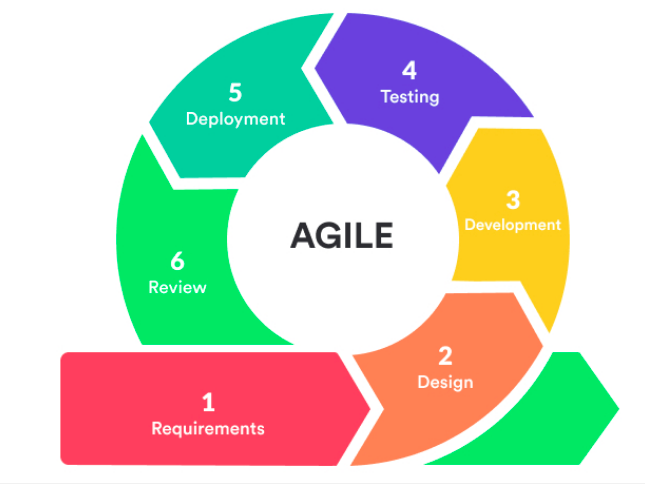
\includegraphics[scale=0.35]{images/Analyse_des_besoins/agile.png}
                \caption{Aperçu des méthodologies agiles pour le développement de logiciels }\cite{agile}
                \label{fig:agile}
            \end{figure}

        \paragraph{Quel framework choisir ?}
        \paragraph{}
        Différentes approches existent pour structurer des processus agiles 
        au sein d'une organisation (en l'occurence: Scrum,
        eXtreme Programming (XP), Adaptive Software Development (ASD), Rapid Application Development (RAD),
        etc).Vous vous demandez probablement comment 
        procéder pour en choisir une. Malheureusement, il n'existe pas de moyen 
        unique de pratiquer le développement logiciel agile. De nombreux facteurs 
        influencent le cadre avec lequel nous choisissons de travailler (tels que: la structure de l'équipe,
        les ressources disponibles,
        les besoins des parties prenantes, ...). 
        \par
        \textit{Ne demandez pas "Kanban vs Scrum". Au lieu de cela, demandez "kanban ou Scrum" 
        ou même "kanban et Scrum"} \cite{Rehkopf}.
        \par
        \paragraph{Scrum}
        \paragraph{}
        \textit{Scrum est un framework qui est utilisé pour implémenter la méthode 
        Agile de développement et de gestion de projet} \cite{Littlefield2017}.
        \par
        Les équipes Scrum s'engagent à livrer les logiciels fonctionnels à des intervalles définis 
        appelés sprints. Leur objectif est de créer des boucles d'apprentissage pour 
        recueillir et intégrer rapidement les commentaires des clients. Les équipes Scrum 
        adoptent des rôles spécifiques, créent des artefacts spéciaux et organisent des cérémonies 
        régulières pour faire avancer les choses. 
        
        \paragraph{Kanban}
        \paragraph{}
        \textit{Kanban est une méthodologie de gestion de projet agile pour le développement de logiciels où l'accent
        consiste à indiquer avec précision le travail à effectuer et le moment où il doit être fait}\cite{skauge}.
        \par
        Kanban consiste à visualiser votre travail, à limiter le travail en cours et à maximiser l'efficacité (ou le flux). 
        Les équipes Kanban se concentrent sur la réduction du temps nécessaire pour prendre un projet (ou une user story) 
        du début à la fin. Ils le font en utilisant un tableau Kanban et en améliorant continuellement leur flux de travail.
        \paragraph{Un mélange de Kanban et de Scrum}
        \paragraph{}
        La méthodologie agile de gestion de projet et le framework Scrum sont basés sur une méthode 
        itérative de livrables du produit. Au lieu d’attendre que le projet soit 100\% finalisé 
        pour le livrer au client, vous délivrez des tronçons “utilisables” du projet au cours du 
        temps. Vous éviterez ainsi de gaspiller des efforts en cas de nécessité de changement ou 
        de problème de communication. Au-delà de l’importance des itérations et des améliorations 
        pour le produit, Scrum s’attache également à améliorer le processus à chaque nouveau cycle.
        \paragraph{}
        Un projet Scrum peut être agencé de différentes manières mais sont toujours présents:
        \begin{itemize}
                \item Product Owner : Il représente les intérêts du client et à ce titre, il a 
                l’autorité pour définir les fonctionnalités du produit final. Dans notre cas, il s'agit de l'URGéo.
                \item Sprint : Scrum utilise des sprints comme intervalles de temps pendant lesquels l’équipe 
                va compléter un certain nombre de tâches. Chaque sprint se termine avec une Rétrospective, qui réunit 
                toute l’équipe afin de partager les retours d’expérience et discuter des améliorations possibles du 
                prochain sprint.
        \end{itemize}

        \paragraph{Pourquoi Agile, Kanban et Scrum ?}
        \paragraph{}
        Nous sommes fixés sur le choix de la méthodologie Agile. Mais concernant la méthode en question,
        on se fait le plaisir de jongler par moments entre Kanban et Scrum. 
        Le tableau \ref{tab:scrumvskanban} fait une comparaison entre ces deux outils et met l'emphase sur leur convergence.
        \begin{itemize}
                \item Scrum est la méthode agile la plus éprouvée et la plus documentée.
                \item Contrairement à la méthode traditionnelle waterfall, l'approche Agile offre une plus 
        grande flexibilité et une meilleure visibilité dans la gestion du projet. 
                \item Les méthodologies Kanban sont continues et plus fluides, tandis que Scrum est basé 
                sur des sprints de travail courts et structurés (qui nous est necessaire par moment).
                \item L'avantage majeur de l'approche Agile est sa flexibilité. Les changements du client et les imprévus 
        sont pris en compte et l'équipe projet peut réagir rapidement.
                \item Le client dispose d'une meilleure visibilité sur l'avancement du projet et peut ainsi l'ajuster 
                en fonction de ses besoins. Le contrôle qualité est permanent. Quant à l'équipe projet, elle peut 
                réagir rapidement aux demandes du client.
                \footnote{
                \url{https://www.planzone.fr/blog/quest-ce-que-la-methodologie-agile}
                }
        \end{itemize}

        \par    
\begin{table}
        \centering
        \begin{tabular}{|p{0.20\linewidth}|p{0.40\linewidth}|p{0.40\linewidth}|}
        \hline
                \textbf{} & \textbf{Scrum}& \textbf{Kanban}  \\
                \hline
                Cadence &
                Sprints réguliers de longueur fixe (ex: 2 semaines)&
                Flux continu
                \\
                \hline
                Méthodologie de publication&
                À la fin de chaque sprint&
                Livraison continue
                    \\
                \hline
                Rôles &
                Product owner, scrum master, development team&
                Aucun rôle requis
                    \\
                \hline
                Indicateurs clés&
                Rapidité&
                Délai d'exécution, temps de cycle, WIP(Work In Progress)
                    \\
                \hline
                Philosophie de changement&
                Les équipes ne doivent pas apporter de modifications pendant le sprint.&
                Le changement peut survenir à tout moment
                        \\

                \hline 
        \end{tabular}
        \caption{Comparaison de Scrum et Kanban} \label{tab:scrumvskanban}
\end{table}
\par
        